\section{Durchführung}
\label{sec:Durchführung}

Das Röntgengerät, welches in Abbildung (2) zu sehen ist, wir über einen Rechner bedient.
Integriert sind eine Kupfer-Röhre, ein LiF-Kristall und ein Geiger-Müller-Zählrohr.
Zu Beginn wird eine Beschleunigungsspannung von $U_B = 35 \si{\kV}$ und ein Emissionsstrom von $I_ 1 \si{\mA}$ eingestellt.

\noindent Um die Bragg Bedingung zu prüfen, wird im Programm ein Kristallwinkel von $\theta = 14$° eingestellt. Das Zählrohr
soll in einem Winkelbereich von $\alpha_{GM} =26$° bis $\alpha_{GM} =30$° laufen.

\noindent Das Emissionsspektrum wird im 2:1 Koppelmodus untersucht. Das Röntgenspektrum soll im Winkelbereich von $\alpha_{GM} =4$° bis $\alpha_{GM} =26$° laufen, und die Intergrationszeit wird auf 5 Sekunden gestellt.

\noindent Für 5 verschiedene Materialen soll das Absorptionsspektrum gemessen werden. Dazu muss ein geeigneter Messbereich ausgewählt werden. 
Die Intergrationszeit wird auf 20 Sekunden gestellt. 
Zuletzt wird von einem Material mit Massenzahl über 80 das gleiche durchgeführt. 

\begin{figure}[H]
  \centering
  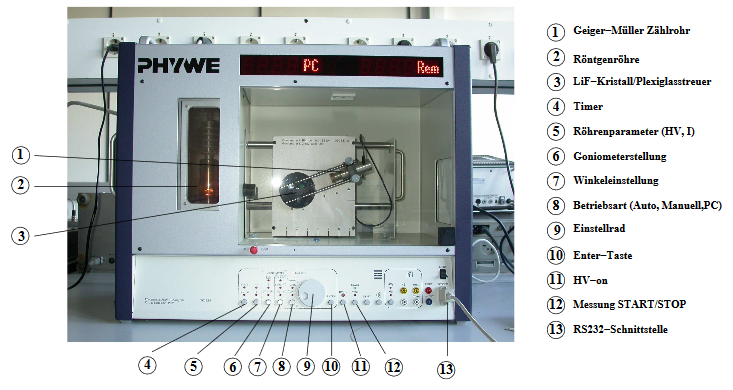
\includegraphics[height=6cm]{geraet.PNG}
  \caption{Das Röntgengerät. \cite[S.4]{kent}}
\end{figure}